\section{Simulation Results}
Figs. \ref{fig:RSBD_Plot2D}-\ref{fig:Single_Body_Simulation_Results_Diff_Load_States} show two sets of simulation results where one leader-follower pair conducts modest turning maneuvers with identical open loop inputs (throttle, steering, and gear shift profiles). The contour maps in Fig. \ref{fig:RSBD_Plot2D} show variations in the terrain friction angle while the terrain cohesion varies accordingly with a correlation coefficient of 0.35. In Fig. \ref{fig:Single_Body_Simulation_Results_Same_Load} and \ref{fig:Single_Body_Simulation_Results_Same_Load_States}, both tractors are towing a 40,000 kg load and shifting between gears 6-9 over a 40 second period. In Figs. \ref{fig:Single_Body_Simulation_Results_Diff_Load} and \ref{fig:Single_Body_Simulation_Results_Diff_Load_States}, all these conditions are maintained except the towed load of the follower is 20,000 kg. From the results in Figs. \ref{fig:Single_Body_Simulation_Results_Same_Load} and \ref{fig:Single_Body_Simulation_Results_Same_Load_States}, it is shown that when two vehicles tow the same load across terrain with similar characteristics, the follower should be able to use the leader's states and control inputs as a nominal trajectory with a controller to make small refinements. However, when large terrain changes occur, an alternative control approach is necessary that computes inputs to minimize the risk of immobilization rather than strictly following a leader's trajectory. The last 20 seconds of simulation results in Fig. \ref{fig:Single_Body_Simulation_Results_Same_Load} and \ref{fig:Single_Body_Simulation_Results_Same_Load_States} support this claim as the slip ratio of the right, outer track exceeds $80\%$. This highlights the ability of the model to predict immobilization as terrain parameters change and justifies how the model could be useful for prediction. The second set of results in Figs. \ref{fig:Single_Body_Simulation_Results_Diff_Load} and \ref{fig:Single_Body_Simulation_Results_Diff_Load_States} simulate the leader and follower under different payloads of 40,000 kg and 20,000 kg and validates that the model has terrain-vehicle dynamics that capture the power-load relationship at the engine output. This can be seen in Fig. \ref{fig:Single_Body_Simulation_Results_Diff_Load_States} where there is a noticeable power output difference between the two vehicles to maintain a similar speed. These simulations were programmed in Matlab and run in real-time for one vehicle after start-up and the clutch is locked.

\begin{figure}[htbp]
\begin{subfigure}{0.5\textwidth}
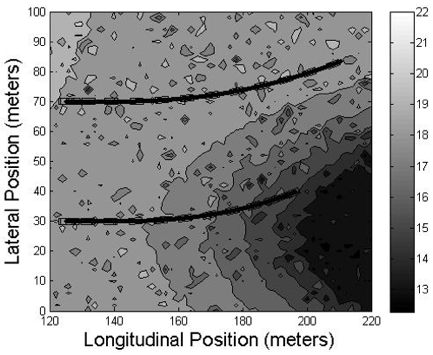
\includegraphics[width = 7.5 cm, height = 6 cm]{Single_Body_Simulation_Results_Same_Load}
\caption{}
\label{fig:Single_Body_Simulation_Results_Same_Load}
\end{subfigure}
\begin{subfigure}{0.525\textwidth}
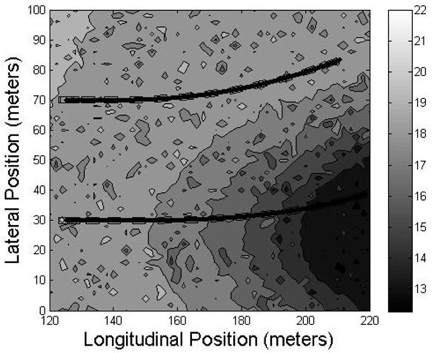
\includegraphics[width = 7.5 cm, height = 6cm]{Single_Body_Simulation_Results_Diff_Load}
\caption{}
\label{fig:Single_Body_Simulation_Results_Diff_Load}
\end{subfigure}
\caption{(a) One leader-follower pair with identical open loop control inputs and towed loads of 40,000 kg. The contour map shows the explicit variation in the friction angle of the terrain (b) One leader-follower pair with identical open loop control inputs. The lead and follower vehicles are towing 40,000 kg and 20,000 kg loads respectively}
\label{fig:RSBD_Plot2D}
\end{figure}

\begin{figure}[htbp]
    \centering
    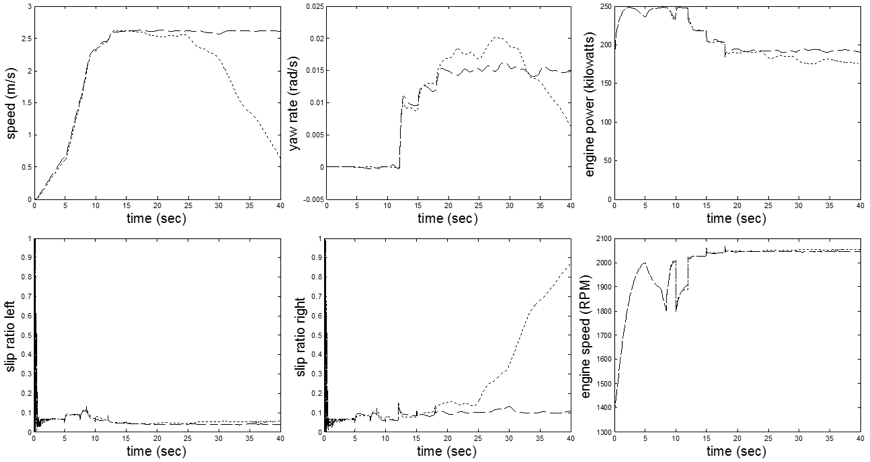
\includegraphics{Single_Body_Simulation_Results_Same_Load_States}
    \caption{Absolute vehicle speed, yaw rate, engine speed and power, and slip ratios for one leader-follower pair. Dashed lines correspond to the lead vehicle while dotted lines refer to the follower}
    \label{fig:Single_Body_Simulation_Results_Same_Load_States}
\end{figure}

\begin{figure}[htbb]
    \centering
    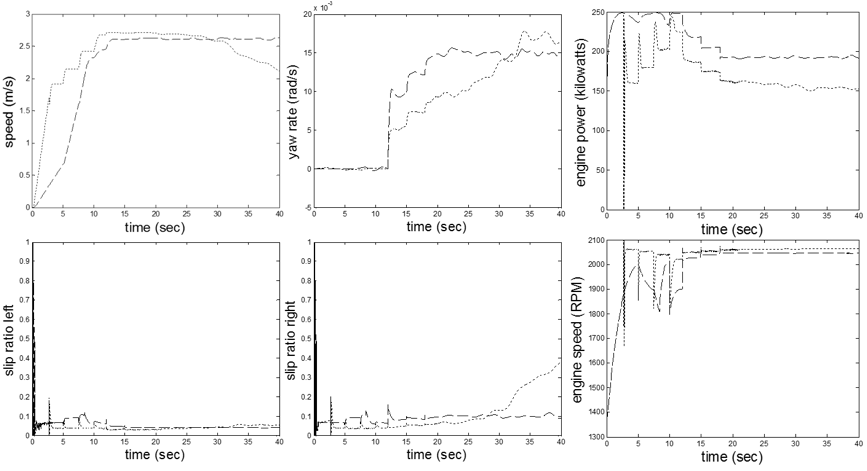
\includegraphics{Single_Body_Simulation_Results_Diff_Load_States}
    \caption{Absolute vehicle speed, yaw rate, engine speed and power, and slip ratios for one leader-follower pair. Dashed lines correspond to the lead vehicle while dotted lines refer to the follower. The follower vehicle is towing 20,000kg}
    \label{fig:Single_Body_Simulation_Results_Diff_Load_States}
\end{figure}